\chapter{Introduzione}
\label{ch:introduzione}

\section{Il premio per il rischio di volatilità}
\label{sec:intro-vrp}

Nei mercati delle opzioni, la volatilità implicita tende sistematicamente a
superare la volatilità che il sottostante realizza successivamente. Questo
differenziale, noto come \emph{Volatility Risk Premium} (VRP), è uno
dei fenomeni più documentati della finanza empirica: chi acquista opzioni
paga, in media, un premio superiore al valore attuariale della protezione
che riceve, e chi le vende incassa tale premio come compenso per
l'esposizione al rischio di volatilità \citep{carr2009variance,
bakshi2003delta}.

Sul mercato delle opzioni Bitcoin il fenomeno assume dimensioni
strutturalmente maggiori rispetto ai mercati azionari tradizionali. Nel
periodo giugno 2021 -- settembre 2024, l'indice di volatilità implicita
DVOL di Deribit ha superato la volatilità realizzata a 30 giorni (stimata
con l'estimatore di Parkinson) nel 93\% delle giornate di negoziazione, con
uno spread medio di 16,2 punti percentuali annualizzati
(Figura~\ref{fig:vrp-btc}). A titolo di confronto, sull'indice S\&P~500 lo
spread analogo è storicamente di 3--4 punti percentuali. La volatilità
implicita media su Bitcoin nel periodo è del 66\%, contro il 16\% circa
delle opzioni su SPY.

\begin{figure}[H]
\centering
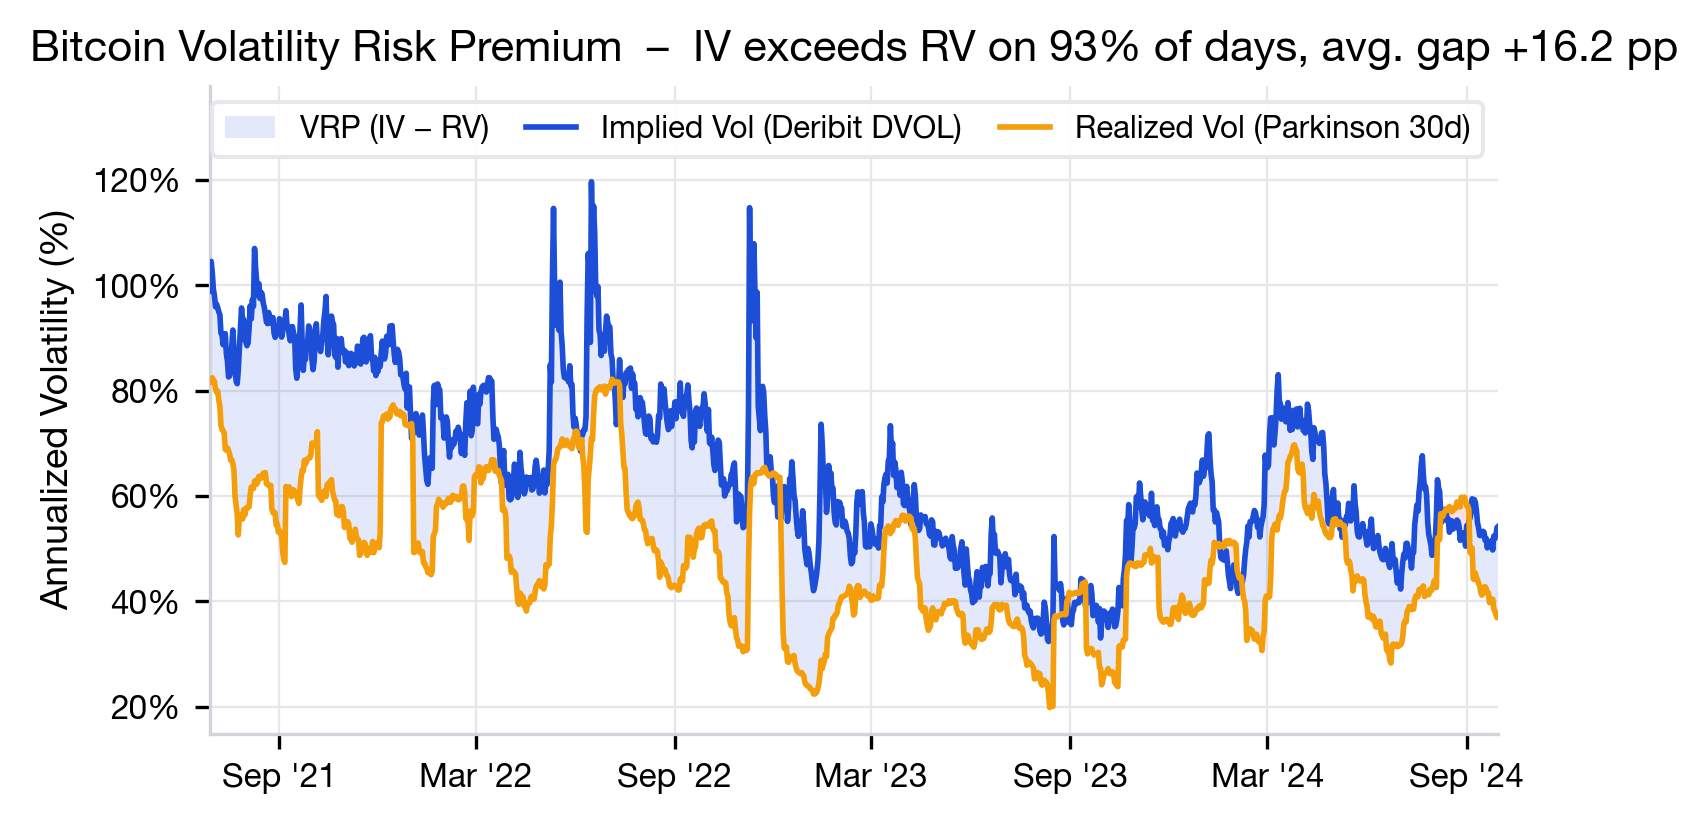
\includegraphics[width=\textwidth]{figures/fig1_vrp.png}
\caption{Volatilità implicita (DVOL) e volatilità realizzata a 30 giorni
(Parkinson) su Bitcoin, giugno 2021 -- settembre 2024. Lo spread medio di
16,2 punti percentuali costituisce il premio per il rischio di volatilità
oggetto di questa tesi.}
\label{fig:vrp-btc}
\end{figure}

Le ragioni strutturali di un VRP così ampio sul mercato crypto sono
riconducibili alla composizione dei flussi: la domanda di opzioni è
dominata dal lato acquisti: investitori retail che comprano call a leva
e operatori nativi del settore (miner, società con tesorerie in Bitcoin)
che comprano put a copertura, mentre l'offerta di volatilità è limitata
dalla scarsità di market maker con capitale dedicato. Il risultato è un
mercato strutturalmente \emph{long gamma} dal lato della domanda, in cui
chi vende volatilità viene remunerato con un premio persistente.

\section{Domanda di ricerca}
\label{sec:intro-research-question}

La domanda di ricerca di questa tesi è la seguente: \emph{il premio per il
rischio di volatilità sulle opzioni Bitcoin è catturabile in modo
sistematico, al netto di costi di transazione realistici, attraverso una
strategia replicabile di vendita di opzioni con copertura delta?}

La risposta richiede di affrontare tre problemi distinti:

\begin{enumerate}
\item \textbf{Selezione}: quale opzione vendere, ogni giorno, tra le
centinaia quotate? Esiste un segnale che discrimini i momenti e gli
strumenti migliori, o la scelta più semplice è anche la migliore?
\item \textbf{Esecuzione e copertura}: come neutralizzare l'esposizione
direzionale al sottostante, e con quale strumento (futures perpetui o
trimestrali), tenendo conto dei costi di ribilanciamento?
\item \textbf{Dimensionamento}: quanta esposizione assumere per trade, in
funzione del capitale, in modo da rendere sostenibili i drawdown di una
strategia short volatility priva di stop loss?
\end{enumerate}

\section{Contributi e metodo}
\label{sec:intro-contributi}

Il contributo di questa tesi non risiede in un modello complesso, ma nel
rigore del processo di eliminazione che conduce alla strategia finale.
Cinque ipotesi progressivamente più sofisticate sono state costruite,
testate e scartate con criteri statistici espliciti:

\begin{enumerate}
\item lo scoring basato sul gap tra densità risk-neutral e densità fisica
(nessun potere predittivo: $\beta < 0$, $p = 0{,}37$);
\item la selezione Premium/DTE (la redditività apparente era interamente
un artefatto dei dati: il 116\% dei profitti proveniva da opzioni illiquide
con bid nullo all'uscita);
\item la modalità multi-posizione (drawdown in-sample del $-49{,}7\%$
durante il crash del 2022);
\item cinque filtri di regime (nessuna correlazione con il PnL per trade
superiore a 0,25 in valore assoluto);
\item lo stop loss (a ogni soglia testata distrugge più profitto dai
trade vincenti di quanto ne salvi dai perdenti).
\end{enumerate}

La strategia sopravvissuta a questo processo è la più semplice possibile:
vendere ogni giorno l'opzione con il vega più alto nell'universo filtrato
($|\Delta| \le 0{,}50$), coprire il delta con futures trimestrali, uscire
al 50\% del premio incassato o a 5 giorni dalla scadenza. Su 35 trade
in-sample (giugno 2021 -- settembre 2023, periodo che include il bear
market del 2022 con un trimestre a $-55\%$ per Bitcoin) la strategia
produce uno Sharpe ratio di 1,75, statisticamente significativo all'1\%
($p = 0{,}007$). Out-of-sample (ottobre 2023 -- settembre 2024) lo Sharpe è
1,52.

Tre elementi rafforzano la credibilità del risultato. Primo, un audit
sistematico del backtest ha identificato e corretto distorsioni che
gonfiavano i risultati preliminari (uscite valorizzate al bid anziché
all'ask, costi di transazione assenti, opzioni illiquide con prezzi
fittizi). Secondo, la validazione cross-asset: la stessa strategia,
applicata senza alcuna riottimizzazione alle opzioni SPY su 14 anni di dati
(147 trade), produce un win rate della gamba opzionaria identico (82\%),
confermando che il meccanismo di cattura del VRP non è un artefatto del
campione Bitcoin. Terzo, l'implementazione live: la strategia è operativa
in paper trading sulla testnet di Deribit, con esecuzione automatizzata
ogni quattro ore, a verifica della replicabilità operativa dell'intera
pipeline.

\section{Struttura della tesi}
\label{sec:intro-struttura}

Il Capitolo~\ref{ch:letteratura} colloca il lavoro nella letteratura sul
VRP e sui mercati delle opzioni crypto. Il
Capitolo~\ref{ch:dati} descrive i dati, il mercato Deribit e
l'infrastruttura di backtest, inclusa l'estrazione della densità
risk-neutral e la costruzione del framework walk-forward. Il
Capitolo~\ref{ch:percorso} documenta il percorso di ricerca: le cinque
ipotesi testate e scartate. Il Capitolo~\ref{ch:strategia} presenta la
strategia finale Top Vega. Il Capitolo~\ref{ch:money-management} sviluppa
il money management: dimensionamento capital-based, sanity check di Kelly,
margini e simulazione Monte Carlo del rischio di rovina. Il
Capitolo~\ref{ch:validazione} contiene la validazione statistica e
cross-asset. Il Capitolo~\ref{ch:paper-trading} descrive l'implementazione
live. Il Capitolo~\ref{ch:limitazioni} discute le limitazioni e gli
sviluppi futuri. Il Capitolo~\ref{ch:conclusioni} conclude.
